% Chapter 3

\chapter{Attraction attention} % Main chapter title

\label{Chapter3} % For referencing the chapter elsewhere, use \ref{Chapter1} 
\newpage

\section{Introduction}

Increasingly, displays are now being installed in most of the locations and most of these displays are full of advertisements and passers-by often try ignoring because or various reasons like, first is ``\emph{information overload}'' that happens on people at some environmental setups, when they enter at place where too much information is delivered and needs to be processed by a single person, and when that is beyond the person capability then they simply ignore them, as Milgram \cite{Information_overload} investigated on information overload stated in his paper that ``\emph{the concept of overload. This term, drawn from systems analysis, refers to a system's inability to process inputs from the environment because there are too many inputs for the system to cope with, or because successive inputs come so fast that input A cannot be processed when input B is presented}'', therefor there are priorities for each input and low priorities are disregarded, for example, disregarding of low priorities inputs is called ``\emph{Banner Blindness}'' in the web, Burke et al \cite{banner_blindness} showed with an experiment using eye-tracking that people tend to ignore banners mostly and have very few number of recalls of the banner contents.

The second reason of ignoring is, that people expect unrelated or uninteresting contents, Huang et al, also investigated and explained that most public displays are ignored and get little glances \cite{When_display}, where at this points Jörg müller and his fellow \cite{display_blindness} investigated on similar effect called ``\emph{Display Blindness}'' they conducted the experiment in university context with two displays first, the iDisplay, that showed information for students, was looked at more often than the other (MobiDiC), that showed coupons for shops. 

This chapter focuses on the comparative study of attracting attention methods with a traditional advertisement in public display and explains the study design and findings, this comparative study was conducted in university Mensa, meanwhile this chapter explains the feedbacks and opinions of people about advertisement in general, whom were interviewed during the study. The purpose of conducting this study was to find out appropriate attracting attention method for interactive advertisement, which are discussed on other chapters.



\section{Attention}
%At the early stages of digital advertisement, they were very interesting for people and people would stand for a while and have a look at the content, simply because it was something new with big screens, and now digital advertisements are increasing everyday and has become very common and it is same as Television ads without sound; therefor most people try to avoid seeing them because it is not interesting for them anymore or is not related to them, some how there is a missing link between people and advertisements. The rise of powerful computers and new technologies in the last decades, we have Interactive advertisements that integrate people involvement to make advertising more effective and usable.

%Designers of Interactive advertisement have focused a lot on the Usability of the them which obviously should not be avoided but many other factors have not been studied deeply that is why it fails to accomplish their main purpose and are treated like simple posters and ignored. Interactive advertisement should be able to Attract and motivate users and finally allow users to interact in a better way. ``\emph{If they capture attention, many displays seem to fail to motivate passers-by to interact, who have other goals in mind. If, finally, the audience has noticed the display and is motivated to interact, interactive displays seem to fail to deal appropriately with the public nature of interaction, where people may avoid interaction in order to maintain their social role and e.g., not look silly}''\cite{DesignSpace}


Every moment we spend alone, with friends in the crowd, in the concert or party our attention keeps tracks of us and make us aware of the environment and we react differently for different stimuli, so ``\emph{Attention is the process that, at a given moment, enhances some information and inhibits other information. The enhancement enables us to select some information for further processing, and the inhibition enables us to set some information aside.}''\cite{Attention}. Attention is influenced by two different processes (Top-Down \& Bottom-Up) \cite{attention1,Attention}. Top-Down process happens when the user has prior awareness (goal) about where to put his/her attention toward, and Bottom-Up process happens when the user has no prior awareness and suddenly by an external stimuli move or change attention toward something. People walking on pathway or walking in a store or waiting in bus station does not have any knowledge or awareness about an Interactive advertisements located there, nor the researchers tend to speak about it for them, at this situation I believe that the attraction of attention should be a Bottom-Up process for the users to drag them to the screens.

The appearance of objects suddenly or moving objects on the screen or contrasting color can capture attention quicker. Yantis and Jonides (1984) demonstrated that the detection of a target in visual search was markedly enhanced when the target was presented as an abruptly\cite{capturingattention}. And the type of contrast change on an object influence priority in visual search, ``\emph{Both the sudden appearance of an object and sudden changes in existing object features influence priority in visual search.}''\cite{Luminance}

Elaine M. Huang, Anna Koster, and Jan Borchers have researched and discussed on ``\emph{When Does the Public Really Look at Public Displays?}''\cite{WhenPublicDisplays}, in this paper they argued that glancing and attention at large displays is complex and is dependent on many factors like Brevity of glances, Positioning of displays, Content format and dynamics, Catching the eye, Display size, this paper provided some recommendations for each of the mentioned factors.

\section{Approaches}
As discussed earlier that Interactive advertisement would need to first attract the passers-by, therefor for the initial phase, three different attracting attention techniques were made that were interactive, and compared them with non-interactive (traditional) advertisement to observe how many of passers-by are being attracted.

John Hardy and his colleague classified the attention level in three categories, (1) Glance, (2) Ignore and (3) Watch. 

\begin{itemize}
\item \textbf{Glance: } This happens when the passer-by apparently turn his/her head and stares the screen for less than 3 seconds.
\item \textbf{Ignore: } This is when the person completely does not look or turn his/her head while passing by the screen.
\item \textbf{Watch: } This is when the person stares the screen for more than 3 second.
\end{itemize}


\subsection{Prototypes}
Three interactive attracting attention method prototypes were developed and their screen backgrounds were set to black.
 
First, was the \emph{Following eye} shown in figure  \ref{fig:Attraction_Attention} these eyes suddenly pop-up when a person passers-by the screen and follows the person by moving its eyeball. The idea behind this is to check if people would react if something abruptly appear on the screen and starts to follow people, This example has very limited movement it is only constraint with limited eye space, but big object with high contrast.

Second, was the \emph{Firework} shown in figure \ref{fig:Attraction_Attention}, it shows different colored and sized firework animation, The application will show a random firework for each person on the scene, there are three blocks of fireworks for three persons, the movement of the person changes the location of the firework. In this example there is more object movement and color changes with high contrast.

Third, was the \emph{silhouette presentation} shown in Figure \ref{fig:silhouttee}, which shows the augmented colored representation of people passing by the screen, the idea is derived from Jorg Müller \cite{LookingGlass}, who has investigated that how passers-by notice the interactivity of the public display by showing different representations of body like Mirrored (1) ``\emph{user silhouettes}'', (2) ``\emph{avatar-like}''representations and (3) ``\emph{real user Image}'', in that paper they concluded that mirroring user image is much more effective to attract users and understand the interactivity of the display, but because of privacy policy and because of social attitude like may be someone does not like to be shown on the screen, only Mirrored silhouettes.

\begin{figure}[H]
    \centering
    \begin{subfigure}[H]{0.3\textwidth}
        \centering
        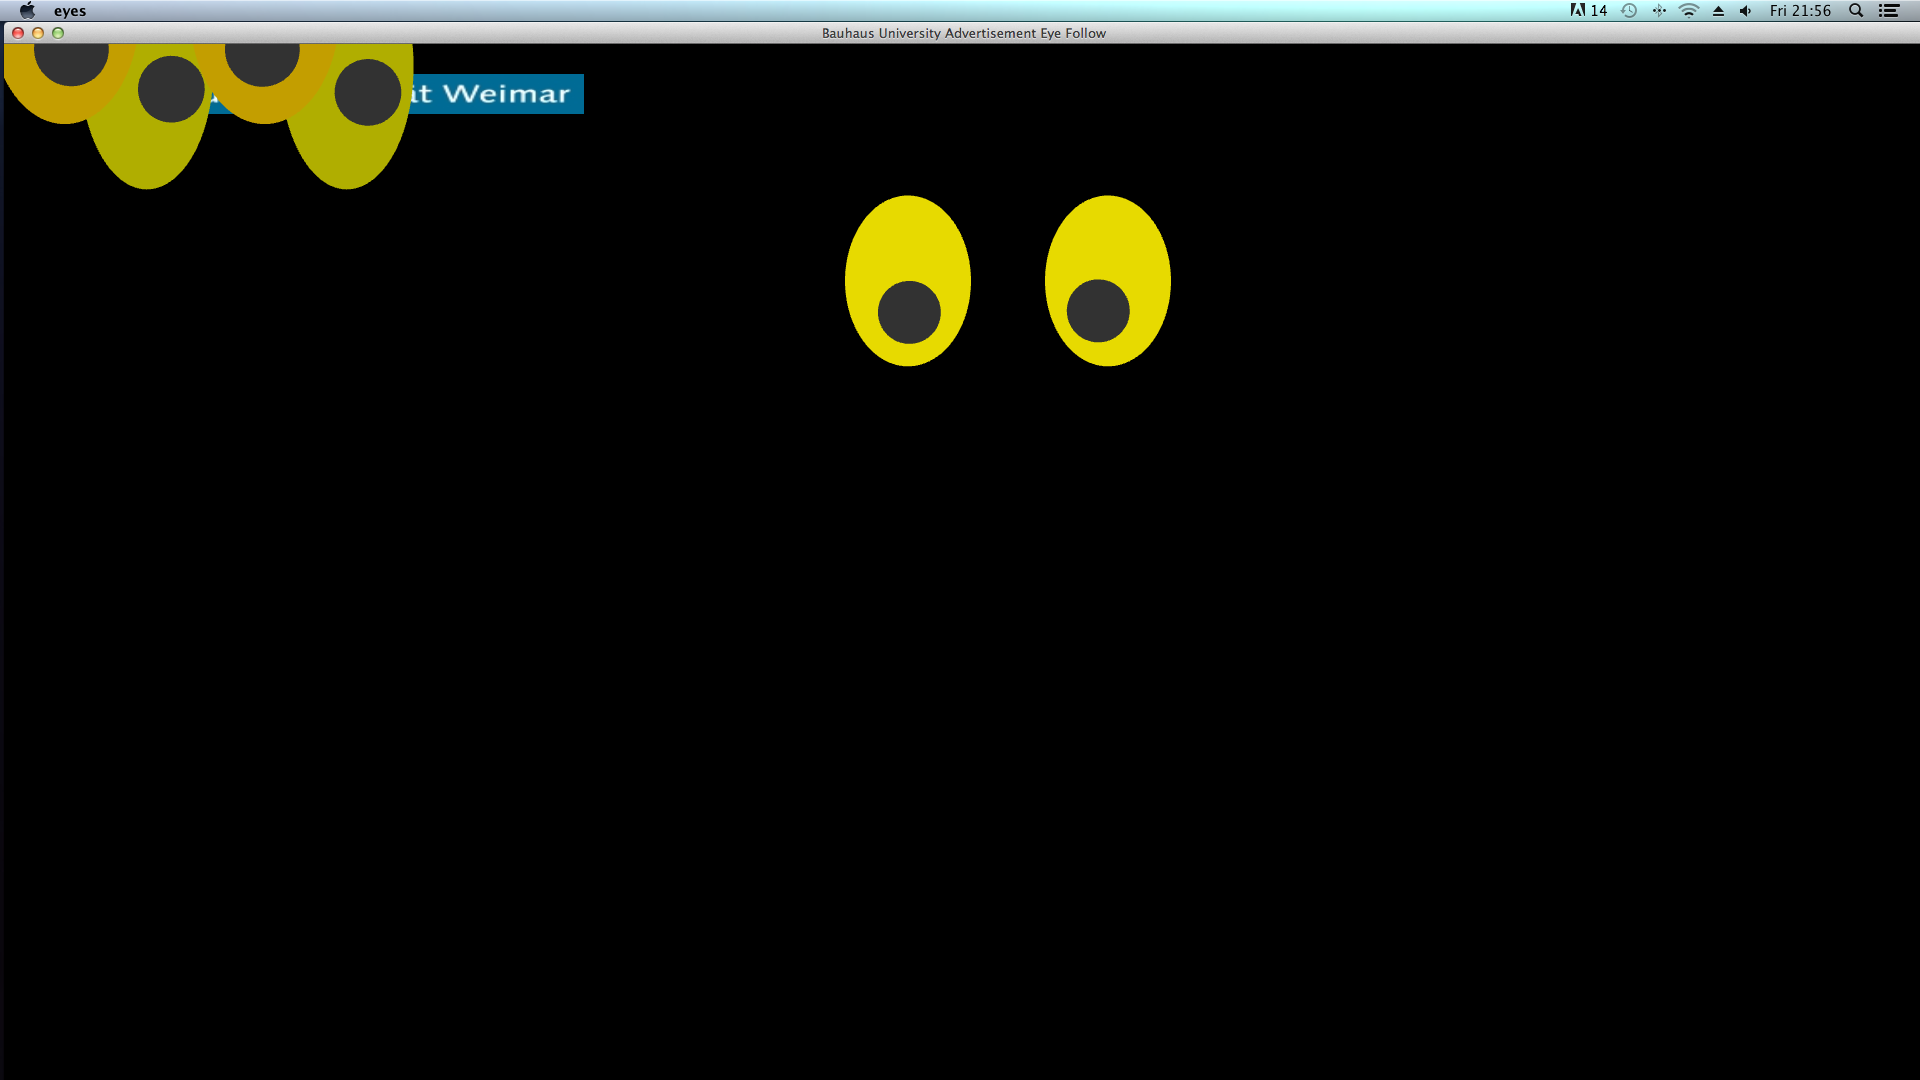
\includegraphics[width=\textwidth]{Figures/3/eyes}
        \caption{Following eyes}
        \label{fig:Attraction_eye}
    \end{subfigure}
    \begin{subfigure}[H]{0.3\textwidth}
        \centering
        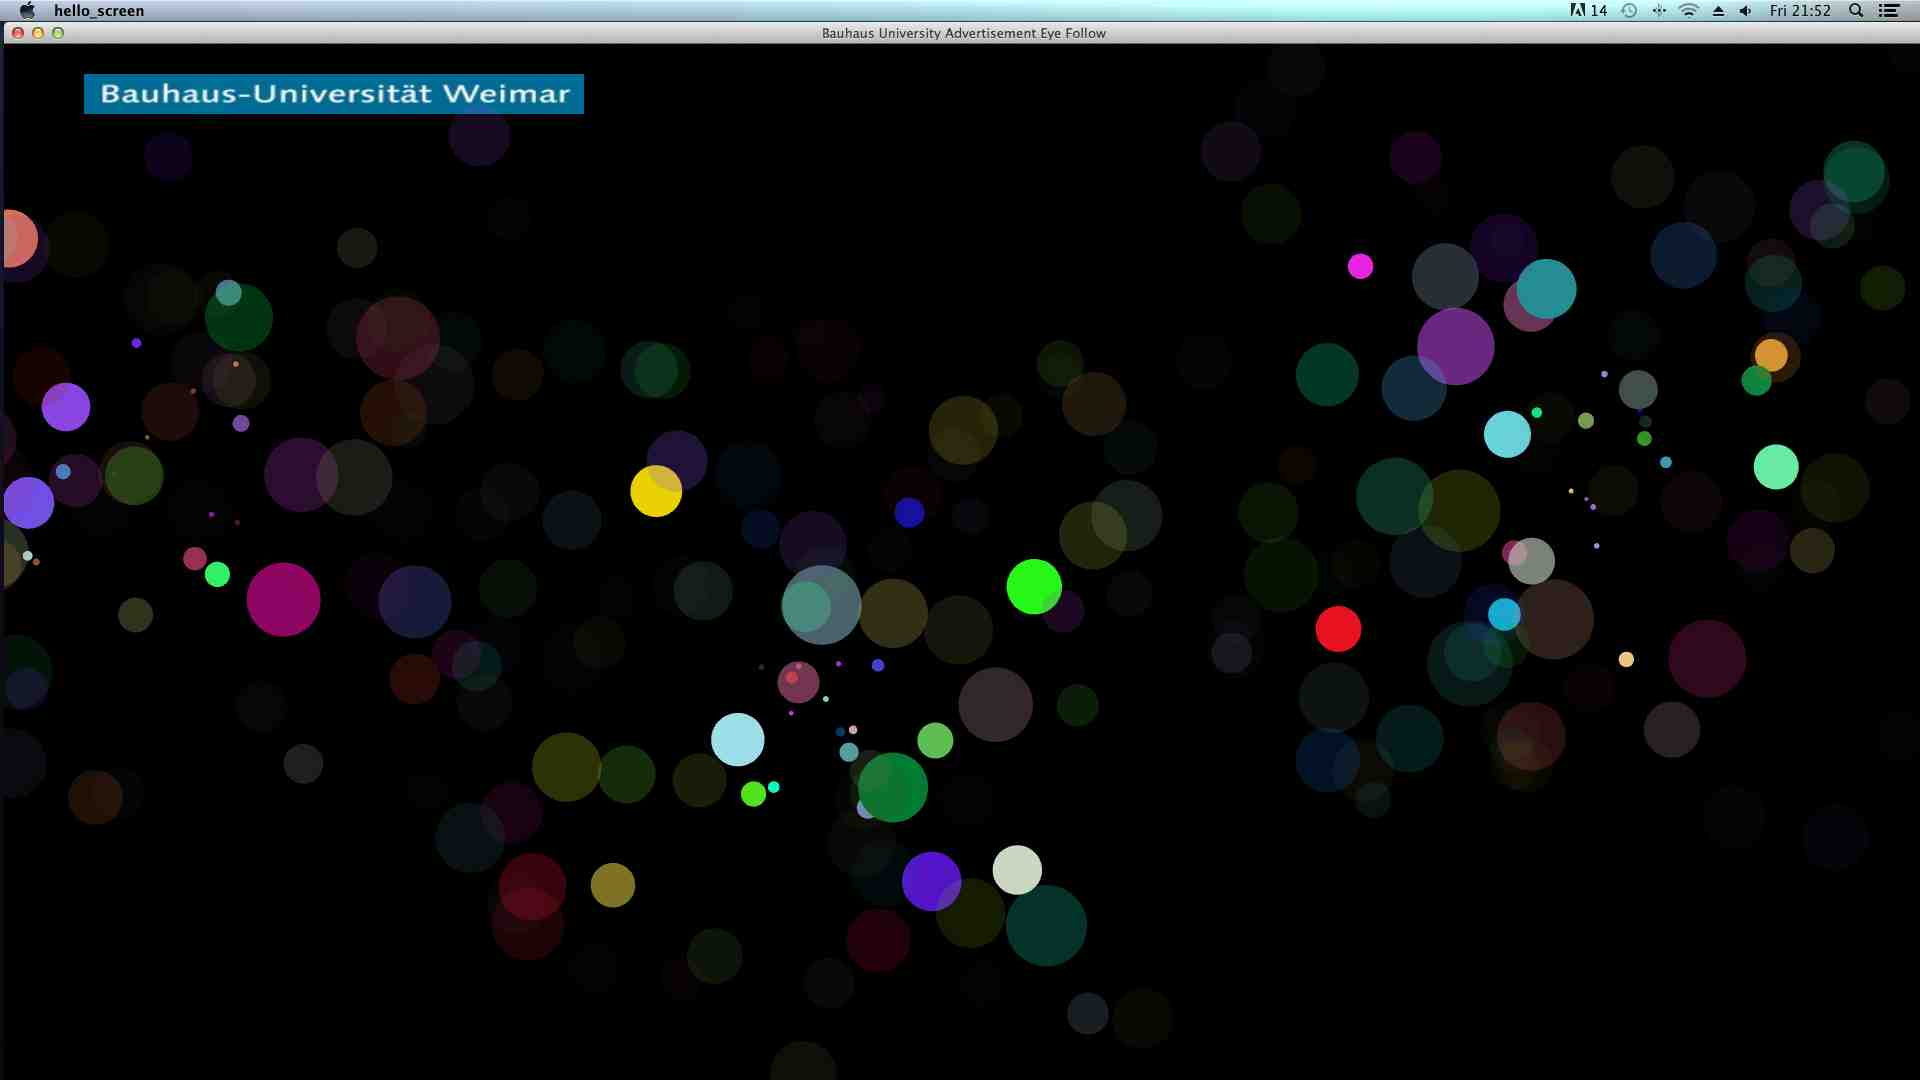
\includegraphics[width=\textwidth]{Figures/3/fireworks}
        \caption{Fireworks animation}
        \label{fig:Attraction_firework}
    \end{subfigure}
      \begin{subfigure}[H]{0.3\textwidth}
        \centering
        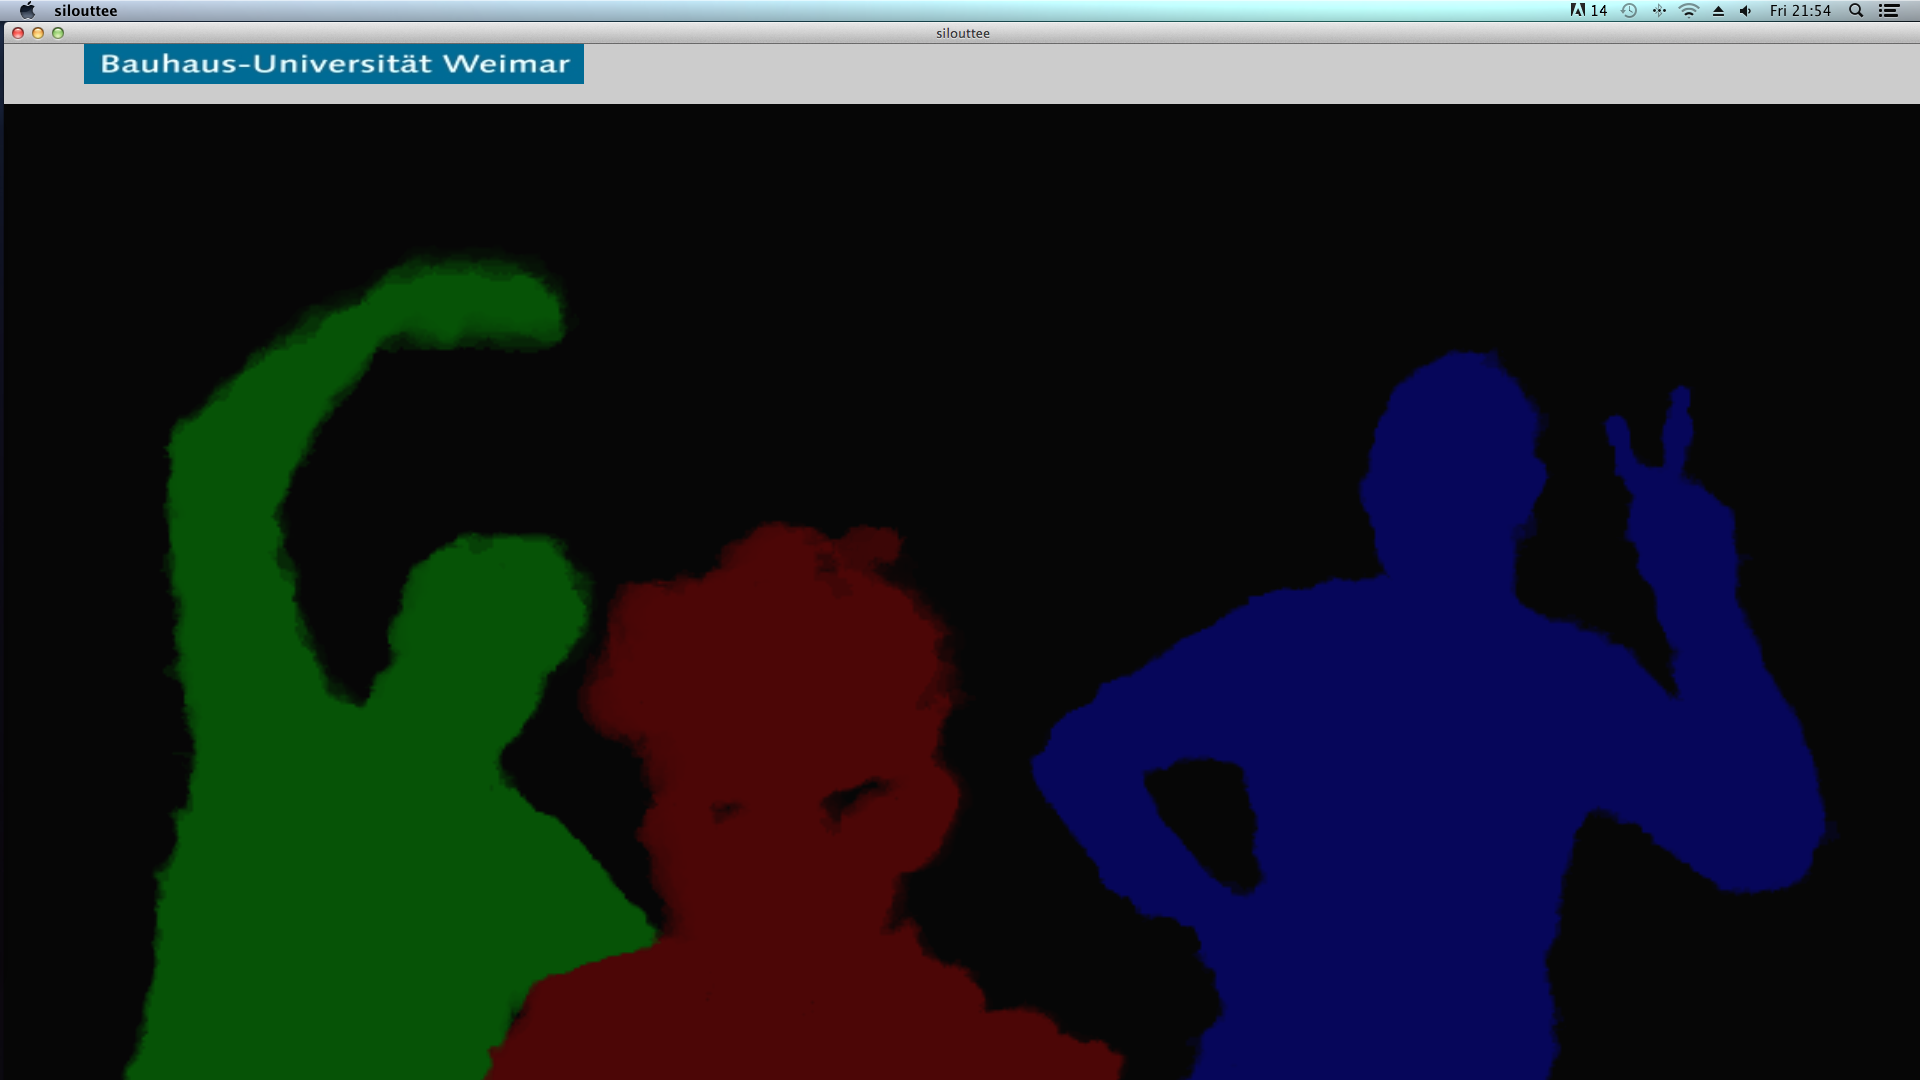
\includegraphics[width=\textwidth]{Figures/3/silhouttee}
        \caption{silhouette}
        \label{fig:Attraction_silhouette}
    \end{subfigure}
    \caption{Attraction attention methods }
    \label{fig:Attraction_Attention}
\end{figure}


Non-interactive advertisement prototype was a traditional style advertisement in which five pages, were in loop in a slideshow, the advertisement pages consisted of pictures and mostly texts about some events in Weimar, the sequence of pages of the slideshow were fixed and would switch from one page to other within about each 15 seconds.

\begin{figure}[H]
\centering
    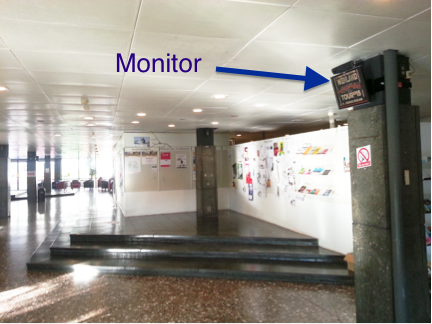
\includegraphics[width=0.5\textwidth,height=4cm]{Figures/3/Kasseturm_monitor}
    \caption{Traditional Advertising }
    \label{fig:kassAdvertising}
\end{figure}


\subsection{Hypothesis}

\begin{itemize}
\item \textbf{H0:} Silhouette representation method and traditional advertising attract same number of passers-by.
\item \textbf{H1:} Silhouette representation method attracts more passers-by than traditional advertising.

\end{itemize}



\section{Study design}
At the beginning, the idea was to conduct some experiment in the lab and investigate about the attention, like doing gaze tracking but it did not suited well for the real life displays in which an already situated display was advertising, therefor that was a nice opportunity to compare our attracting attention methods with the traditional advertising.  

\subsection{Participants}
Participants were random from university students or employees, mostly consisted of students and teachers, the participants were observed that passed in front of the display, The participants who passed from the backside of the display were not taken in consideration. None of the participants knew about the attracting attention conditions in advance.

\subsection{Location}
The study was conducted in university Mensa, this location was an ideal location because many students, teachers and university employees go for having lunch and taking coffee breaks and the Mensa gets crowded. 14-inch display, which was previously used for advertisement in Mensa by Kasseturm\footnote{Kasseturm: \url{http://www.kasseturm.de/}, last accessed: 26 May 2016}, was used to deploy our methods.

\subsection{Procedures}
The study was conducted for four continues days, and each day only one method was displayed on the screen for two hours at 14:00 o’clock, The first day of the study was the passive mode of the screen, where traditional advertisement was displayed and the next three days were the interactive mode of the screen, where the attracting attention methods were shown. One person was responsible for observing and noting the glances made by the passers-by and also noting interesting behavior of people toward the screen. The other person was responsible to take interviews from the passers-by that glanced at the screen and get more feedbacks of the advertisement in general.

\subsection{Data gathering}
Data gathering consisted of direct observation of passers-by from 14:00 – 16:00 for each individual day and interviews were taken which was recorded. 

\subsubsection{Observation}
Observation was used to count the number of glances the passers-by make at the screen while pass from the front of the screen. A small pilot study was conducted for the observer to find an appropriate location in the Mensa setup to be able to count people and glances without being noticed by passers-by.

%The first day, which was a normal advertisement, did not require Kinect Camera, but in order to have same environment for all the days, The camera was installed on top of the monitor to look similar as the other interactive feature.


\begin{figure}[H]
\centering
    \begin{subfigure}[H]{0.45\textwidth}
        \centering
        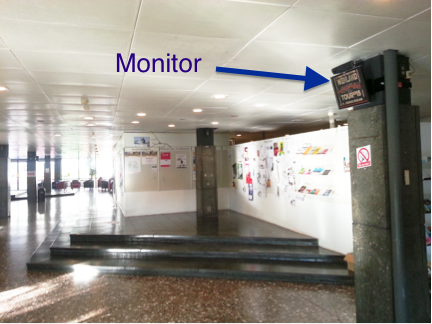
\includegraphics[width=\textwidth,height=4cm]{Figures/3/Kasseturm_monitor}
        \caption{Kasseturm Advertising monitor.}
        \label{fig:kasseturm}
    \end{subfigure}
    \begin{subfigure}[H]{0.45\textwidth}
        \centering
        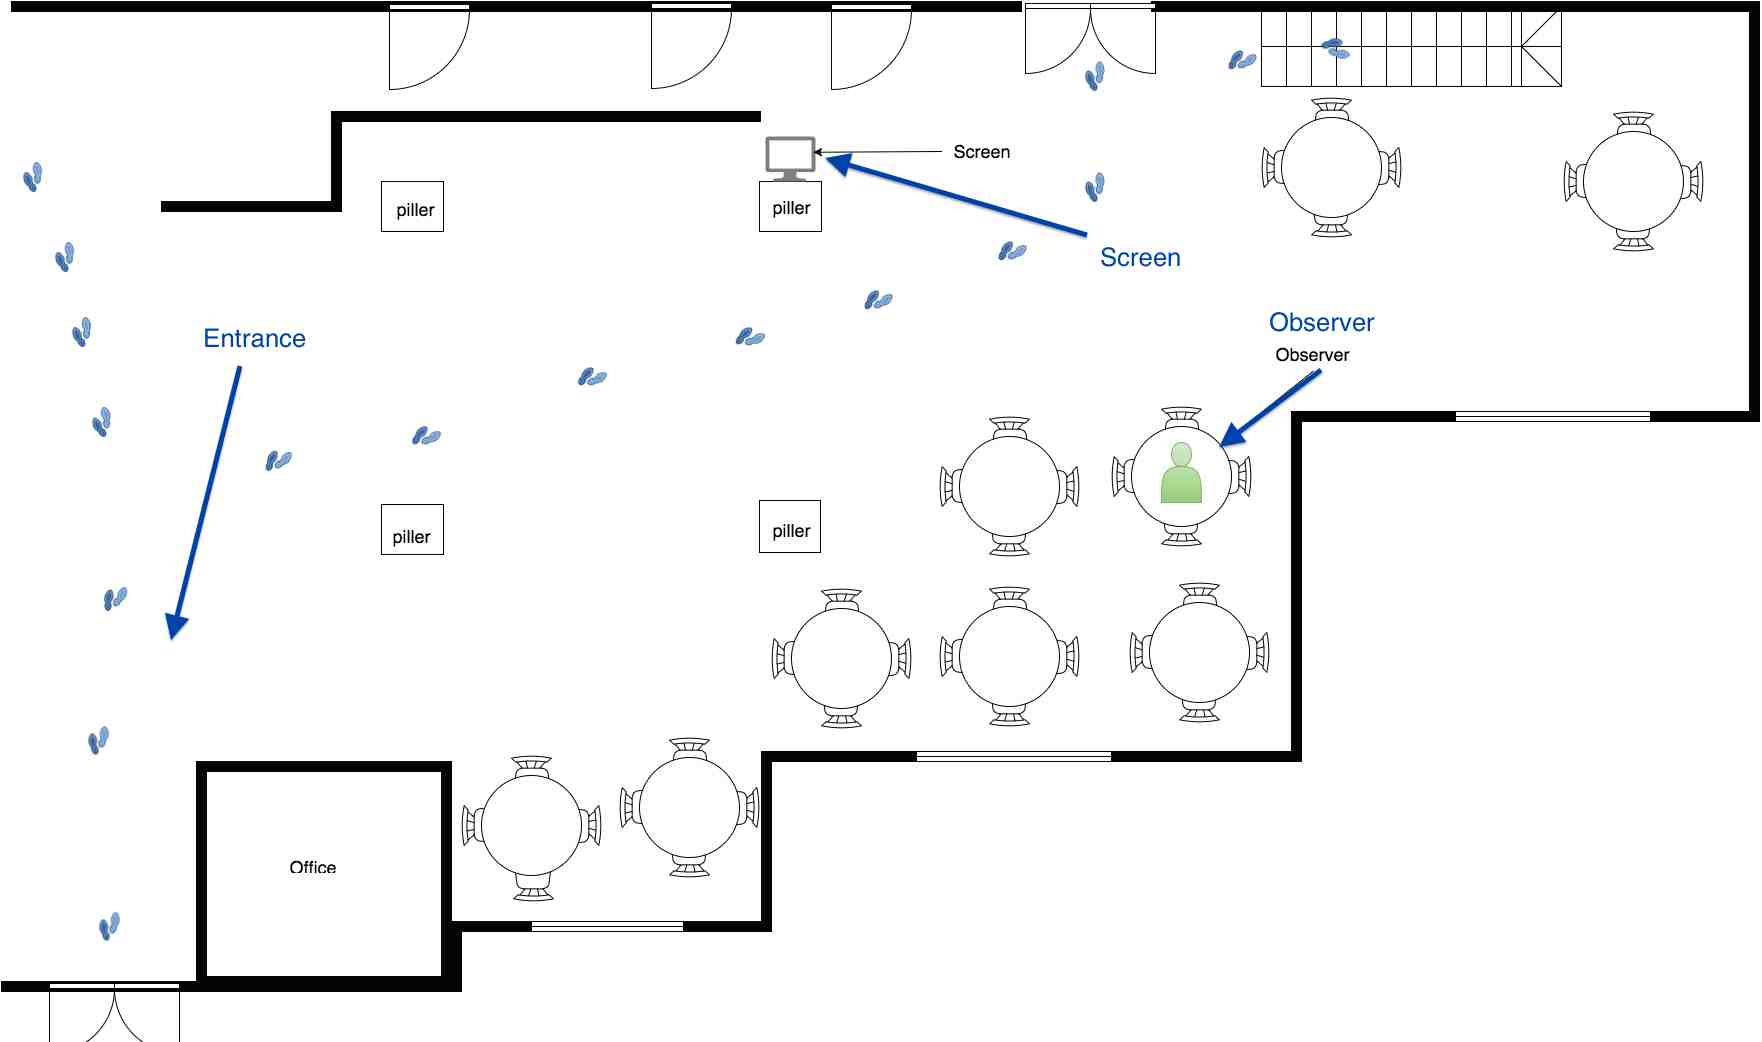
\includegraphics[width=\textwidth,height=4cm]{Figures/3/mensa_setup}
        \caption{Mensa ground floor plan.}
        \label{fig:mensasetup}
    \end{subfigure}
    \caption{University Mensa }
    \label{fig:observation_env}
\end{figure}


A sheet was provided to the observer to note each 5 min time stamp for two hours, specific letters were defined to detect Male, Female, Unknown gender and at the same time who were in a group and individual and who glanced to the screen. \hilight{fix appendix}
%See \ref{AppendixA}.1

As stated before that observer did one small pilot study to locate a good location and be able to count and note in the sheet, beside that, he was told to write notes when he observes something interesting during the period.


\begin{figure}[H]
    \centering
    \begin{subfigure}[H]{0.45\textwidth}
        \centering
        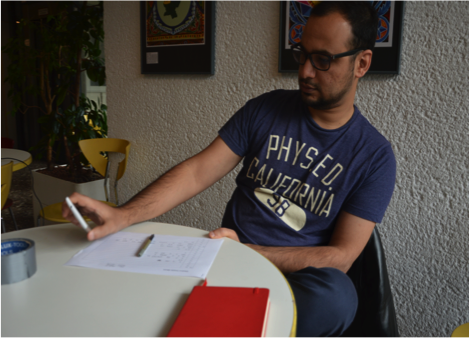
\includegraphics[width=\textwidth,height=4cm]{Figures/3/hamid}
        \caption{Hamid Sabri as an observer.}
        \label{fig:hamid}
    \end{subfigure}
    \begin{subfigure}[H]{0.45\textwidth}
        \centering
        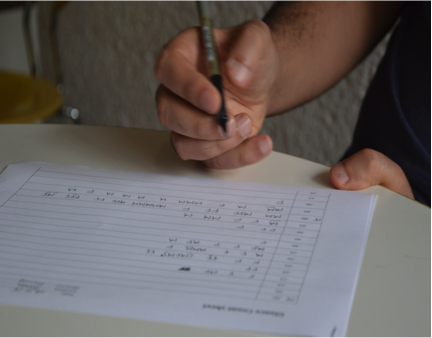
\includegraphics[width=\textwidth,height=4cm]{Figures/3/observer}
        \caption{Observer is taking notes on the data sheet.}
        \label{fig:Observer}
    \end{subfigure}
    \caption{Observation method}
    \label{fig:observation_env}
\end{figure}


\subsubsection{Interviews}

During all four day of the observations, 16 interviews were taken from people inside Mensa to get general opinion about advertisement and people preferences what they like and what they avoid about advertisement. Responders were asked to sign the consent form because the interviews were tap recorded for later analyzing.  Each interview took around 6 minute in average. All interviews were transcribed separately for further data analyzing.

See \hilight{fix appendix}
%\ref{AppendixA}.2 for consent form and  \ref{AppendixA}.3 for the questionnaire.



\section{Findings}
The findings are categorized as bellow.


\subsection{Observation findings}
Observational data for attention level of passers-by was collected and summarized as bellow.


% table
\begin{table}[H]
\caption{Cross tabulation of deployment and attention level }
\label{tab:crosstabulation}
\centering
\resizebox{0.8\textwidth}{!}{ 
\begin{tabular}{| l | c | c | c |}
\toprule
\tabhead{Methods} & \tabhead{Glanced (\%)} & \tabhead{ingnored (\%)} & \tabhead{Total } \\
\midrule
\textbf{Traditional}     & 9  (\%7.6)     &   109 (\%92.3)     &   118\\
\midrule
\textbf{Silhouette }     & 22 (\%15.82)    &   117 (\%84.7)     &   139\\
\midrule
\textbf{Following eye}   & 10 (\%12.98)   &   67  (\%87)       &   77\\
\midrule
\textbf{Firework }       & 6  (\%10.1)    &   53  (\%89)       &   59\\
\bottomrule
\end{tabular}
}
\end{table}

As can be seen from the table above, Silhouette attention attraction technique received the highest number of glances 22 out of 139 compared to other techniques, Following eye technique was the second most attracted technique probably because of its contrasting color and funny.

To find the statistical significant difference between traditional screen and these three methods Chi-squared test was applied as bellow.

% table
\begin{table}[H]
\caption{Cross tabulation of Following and traditional attention level }
\label{tab:Followingtraditional}
\centering
\begin{tabular}{| l | c | c | c |}
\toprule
\tabhead{Method} & \tabhead{Glanced} & \tabhead{ingnored} & \tabhead{Total } \\
\midrule
Traditional     & 9      &   109      &   118\\
\midrule
Following eye   & 10     &   67       &   77\\
\midrule
\textbf{Total } & 19     &   176      &   195\\
\bottomrule
\end{tabular}
\end{table}

Performing the ch-squared test on above table, ${\chi}^2$ \emph{(1, N=195)=1.522, p >.05 (p=.21)}, it suggests that there is no significant difference to attract passers-by between following-eye method and traditional screen 


% table
\begin{table}[H]
\caption{Cross tabulation of Firework and traditional attention level }
\label{tab:fireworktraditional}
\centering
\begin{tabular}{| l | c | c | c | }
\toprule
\tabhead{Method} & \tabhead{Glanced} & \tabhead{Ignored} & \tabhead{Total } \\
\midrule
Traditional     & 9      &   109      &   118\\
\midrule
Firework        & 6      &   53       &   59\\
\midrule
\textbf{Total } & 15     &   162      &   177\\
\bottomrule
\end{tabular}
\end{table}

After the ch-squared test,${\chi}^2$\emph{(1, N=177)=0.328, p >.05 (p=.56)}  suggests that there is no significant difference to attract passers-by between Firework method and traditional screen.

% table
\begin{table}[H]
\caption{Cross tabulation of Silhoutte and traditional attention level }
\label{tab:traditionalsilhoutte}
\centering
\begin{tabular}{| l | c | c | c | }
\toprule
\tabhead{Method} & \tabhead{Glanced} & \tabhead{ingnored} & \tabhead{Total } \\
\midrule
Traditional    & 9      &   109      &   118\\
\midrule
Silhouette     & 22     &   117      &   139\\
\midrule
\textbf{Total }          & 31     &   226      &   257\\
\bottomrule
\end{tabular}
\end{table}

After performing the ch-squared test, ${\chi}^2$\emph{(1, N=257)=4.046, p < .05 (p=.04)}, it suggests that Silhouette representation attracts more passers-by than traditional advertising screen. Based on this finding, \emph{H0} is rejected because the attention level of traditional advertising and interactive silhouette presentation are not the same, silhouette presentation attracts statistically more passers-by thank traditional, as a result H1 is accepted.



\subsection{Interview Findings}
Interview transcripts were individually coded to generalize the responder's opinions on the advertisements. I created two main sections from the interviews that what makes a Good Advertisement, and what makes a Bad Advertisement and related all responses to these sections a lot of codes were analyzed and grouped together to make sub sections and sub-sub-sections.

\subsubsection{Good Advertisement}
A lot of categories have been found after coding the interviews the chart in Appendix A, show all the categories and sub categories with the correspondent code from the interviews and even some codes were directly also placed as a category instance. The bellow list describes some of the important categories retrieved from the diagram.
\hilight{reference the code diagram}

\begin{enumerate}
\item \textbf{Content} \\
Responders like to have more funny contents than any other strict informational advertisement; As responders replied like this, ``\emph{just make it funny like make a joke or something but something in a very good one that is really difficult}'', ``\emph{it should be very not very serious?, ?Yeah mostly I like funny things that the main concept is shown in different way like in funny things}'',``\emph{I like advertisement that are somehow have humor}''.

At the same time responders would like to see some useful, true, sensible facts and main idea of advertisement; ``\emph{an offer if it is clearly mentions that okay that you save this much or you get this or that, that is like a clear message}'',  ``\emph{You have to focus on the main things that will happen in the event which will attract people will come.}'' 

Furthermore, contents of advertisement should be small and understandable; ``\emph{the advertisement should be clear too}'', ``\emph{when you have too many numbers and too much to read then it is confusing}'' ``\emph{Add some pictures based on the advertisement what do you want to show.}'', ``\emph{Not many text in advertisement}'',``\emph{Have a good design, not too crowded with information}'', ``\emph{Well defined subject, and shorter contents, because we don't like reading long things usually no  body likes to read}''. 

Another important thing was context Based contents, the users liked to see things related to their surroundings; ``\emph{if I am standing near a shopping center it should tell me that what kind of shops are there and what I could buy from there.}'' ``\emph{It should show movies of the actor I like}''. 
		
		
\item \textbf{Creativity} \\	
People like to see very new and creative things happening in advertisement; ``\emph{something that catches your attention in a way that you haven't seen before}'' , ``\emph{like seeing something out of ordinary}'' . Introducing new ideas, artistic; ``\emph{as I am musician you know kind of creative person I like if it something special inside not it is just like for example if it is advertisement of milk }'' , ``\emph{Which can be something un-expectable probably also }'' , ``\emph{in general I would say yes as long it gets creative}'' 

\item \textbf{Style} \\	
The style of advertisement plays key role in terms of color and size as stated by responders; ``\emph{may be should be more should be more colorful?, ``\emph{my eyes are attracted to so hard things unless there is something big enough things }'', ``\emph{Use the bright color.}'' ,``\emph{You have to be clever in using colors okay because color mismatch does not attract the eyes}'', ?when it is really just like an art like you have a picture you some impression or illusion}''.

\item \textbf{Location} \\	
Responders like to see advertisement while they are on the way, they don?t get annoyed if advertisements comes on their way and some probably take a look to them too, but heavily they do not like advertisement while they are at home or watching program in TV or Internet, ?I think the street is better?

\item \textbf{Interactivity} \\	
Some liked to have some sort of interactivity to experience like playing games; ``\emph{it is good like if you have a game, it would better to have a preview of the game on the screen or just like something like even people could interact with it like get an experience of the game}'', ``\emph{if the screen will also be interactive so you can interact with the with the something you are advertising.}''

\item \textbf{Mean} \\
Different means were mentioned like larger screen, sound, banners for good influential advertisement.

\item \textbf{Motivation} \\
One of the responder pointed that the advertisement should motivate users in a natural way and should be from unbiased point of view; ``\emph{I prefer to buy in a natural way. The company should know who are using their product the power users who that have a lot of influence you know if you have good connections with the guitarists who have like actually like you know people listen to his opinion I think you have to reach out to the guitarist but once you know the guitarist is gaining something from that guitar maker then I don?t trust that company, It should be like completely unbiased, I think that is the kind of advertisement I listen to. }''. 

Others suggest that advertisement must motivate for healthy diet and sport; ?if it reminds me to do stuff like do more sport or eat healthier or anything that has a good purpose?

\item \textbf{Other categories} \\
Many other categories were also extracted for a good advertisement like Goal of advertisement, Audience, Purpose and motivation, for more detail look at appendix A.
		
\end{enumerate}



\subsubsection{Bad Advertisement}
The bellow categories were derived from the interviews that make an advertisement feel or look bad, and we should not avoid using in advertisements.
\hilight{reference the code diagram}

\begin{enumerate}
\item \textbf{Style} \\
There exist different styles that advertisement makers follow but texts or photos are blinking; ``\emph{try not to use anything would be blinking okay because that is really annoying okay because even so if you are not looking at it is still effecting}''. Using of mismatched colors in advertisement is certainly a bad idea; ``\emph{color mismatch does not attract the eyes}''.

\item \textbf{Annoyance} \\
Most of the responders felt annoyed by almost all advertisements because they contain some sort of similar features like repetitions; ``\emph{it should not be like repeating itself over and over and over again}'', ``\emph{I like advertisement apart from watching it again and again}'',``\emph{Hmm if I see the same advertisement again and again that is annoying.}''. 

Other feature is destruction, which does not allow a person on focusing on something; ``\emph{Not just like something popping up in front of your face}'', ``\emph{for example in middle of the serial or a movie that i am watching and an advertisement that is I don't like because it makes me destructed now I just can't focus on things for view minutes you have to leave what ever you were}''

\item \textbf{Motivation} \\
Advertisement in general motivate people in their own way to attract customers, which people make not like it, for example sudden appearance of something in the screen or what users do not like to see but they are forced to see; ``\emph{usually you are forced to see them because you are watching something or doing something and suddenly it comes and it disturbs you}'', ``\emph{it is trying to convince me of something only for to consume or buy and then I mean I don't want}''

\item \textbf{Content} \\
Some advertisements exaggerate on their products or even say lie; ``\emph{it is like magnificent thing and nice pen okay and then it is just a pen, okay}'', ``\emph{They are all lies. Showing inappropriate content are heavily disliked;}'' ``\emph{whenever I go and access the Internet okay A lot of advertisement comes to my face and most of them are inappropriate.
Stuffs like that I don't like them at all for example some perfume ad which would the a woman in a very degrading position or for example mocking someone believe or something just to catch the attention that is probably to offend people that is what would annoy me a lot. The use of ugly and old people is also not welcomed.}''

\item \textbf{Duration} \\
Long lasting advertisement are always boring and waste of time, most of the responders said that they would prefer short advertisements.

\item \textbf{Other categories} \\
Many other categories are also extracted from the interviews like location, Confusing advertisement, Controversial ads, amount of ads and types of ads that were not liked by responders. For more information.

\end{enumerate}

\section{Conclusion} 
As a result this research takes all the considerations and concerns about the nature of traditional advertisement and what the passers-by think that could be good for the advertisement in terms of attractiveness, content and many other factors described in this chapter. A good advertisement from people points of view is an advertisement that provides most relevant content to the theme and environment, is short and precise, should have creativity and some kind of interactivity. Many other negatives aspects should be avoided like having a bad style, being annoying and putting non-context contents.

Regarding the attracting attention, among other techniques the silhouette representation statistically attract more passers-by because of a higher number of glances, and also based on the findings of J. Müller\cite{LookingGlass} silhouette representation is a well accepted presentation of people that can by interesting, joyful and obviously more attractive. This technique would be used for attracting attention for coming interactive advertisement both for (mobile and body). 



